\documentclass{article}
\usepackage{amsmath,amssymb,amsfonts}
\usepackage{xcolor}
\usepackage{amsfonts,amsmath}
\usepackage{color}
\usepackage{tikz}
\usetikzlibrary{calc}
\usetikzlibrary{shapes.geometric}
\usetikzlibrary{shapes,decorations,arrows,calc,arrows.meta,fit,positioning}
\tikzset{
	-Latex,auto,node distance =1 cm and 1 cm,semithick,
	state/.style ={ellipse, draw, minimum width = 0.7 cm},
	point/.style = {circle, draw, inner sep=0.04cm,fill,node contents={}},
	bidirected/.style={Latex-Latex,dashed},
	el/.style = {inner sep=2pt, align=left, sloped},
	square/.style={regular polygon,regular polygon sides=4}
}

\newcommand{\myassetnode}[5]{\node[state,circle] (#1) at (#2,#3) {#4};
	\node[state,square,scale=0.5, fill=white!100] (#1asset) at (#2+0.3, #3-0.3) {#5};
}

\begin{document}

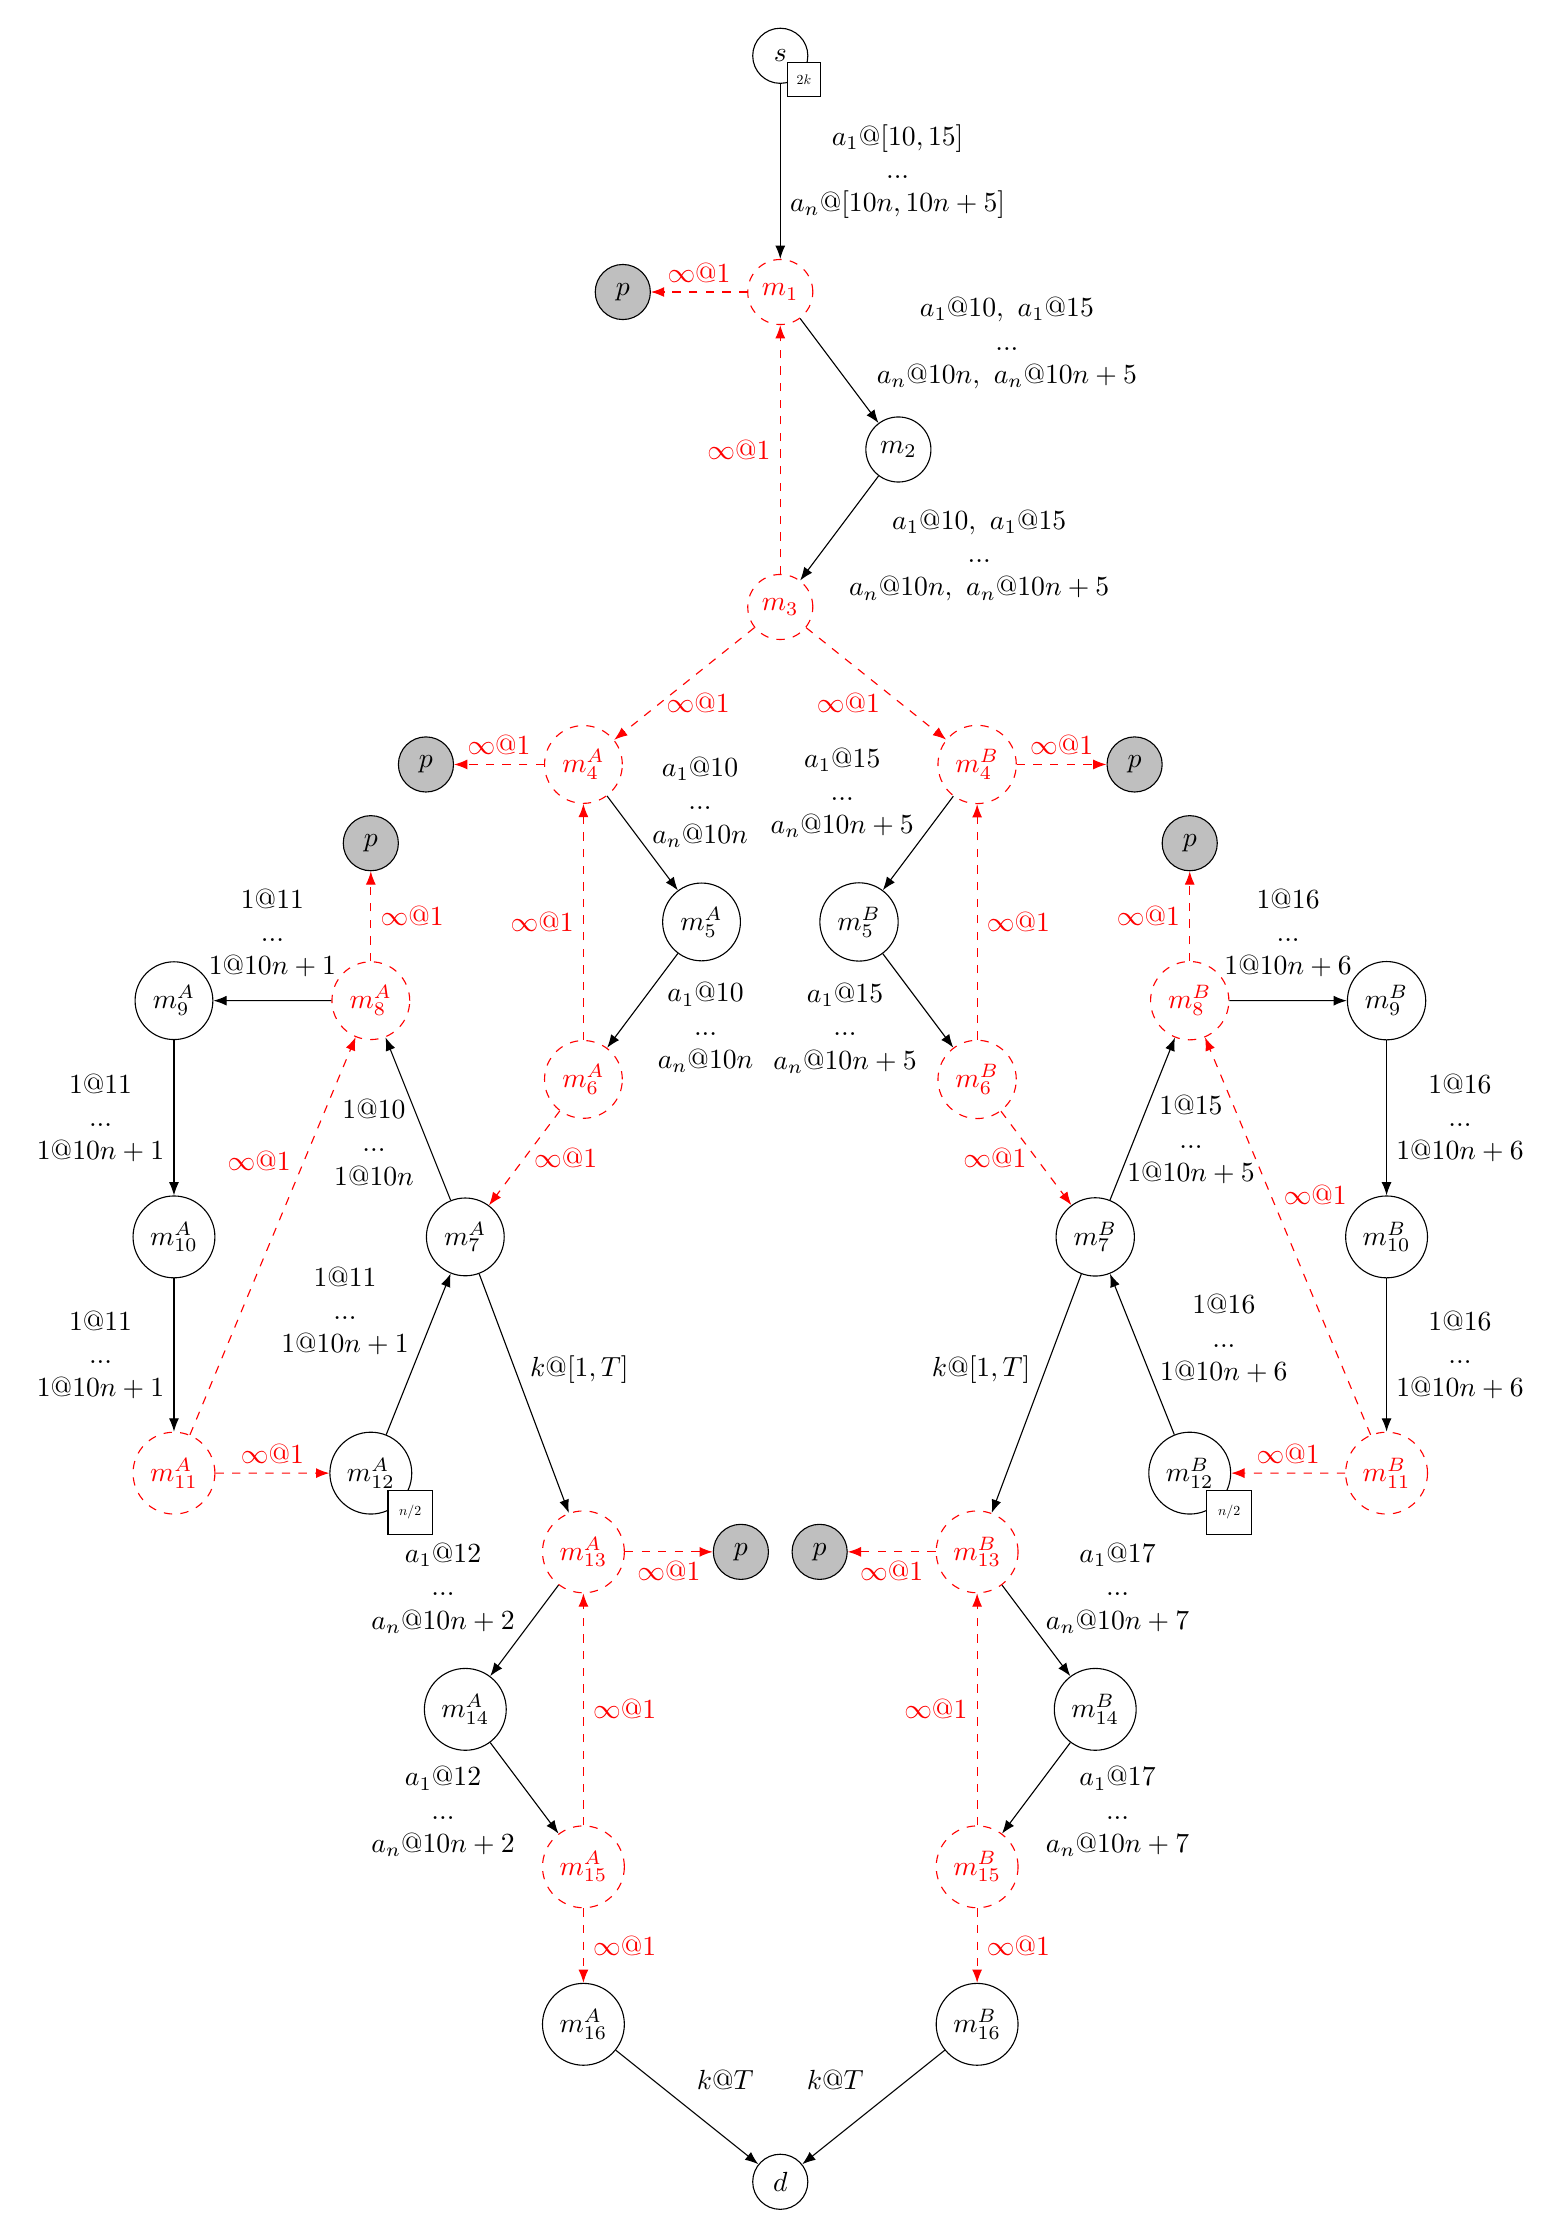
\begin{tikzpicture}
	\myassetnode{s}{0}{0}{$s$}{$2k$}
	% gadget 1: guarantee that each debt is paid at a time divisible by 5
	\begin{scope}[xshift=0cm, yshift=-3cm]
		\node[state,circle,draw=red, dashed, text=red] (m1) at (0,0) {$m_1$};%
		\node[state,circle,draw=black, text=black, fill=lightgray] (t01) at (-2,0) {$p$};%
		% invisible out-node
		\node[state,draw=none] (m1_out) at (-2,0) {};%
		\path[draw=red, dashed, text=red] (m1) edge[draw=red] node[above] {$\infty@1$} (m1_out);	
		\node[state,circle] (m2) at (1.5,-2) {$m_2$};%
		\node[state,circle,draw=red, dashed, text=red] (m3) at (0,-4) {$m_3$};%
		% invisible out-node
		\path[draw=red, dashed, text=red] (m3) edge[draw=red] node[left] {$\infty@1$} (m1);	
		\path (m1) edge node[align=center, yshift = -10pt, xshift = 10pt] {$a_1@10,~ a_1@15$\\$...$\\$a_n@10n,~a_n@10n+5$} (m2);
		\path (m2) edge node[align=center, yshift = 10pt] {$a_1@10,~ a_1@15$\\$...$\\$a_n@10n,~a_n@10n+5$} (m3);
		\path (s) edge node[align=center] {$a_1@[10, 15]$\\$...$\\$a_n@[10n, 10n+5]$} (m1);
	\end{scope}
	% gadget 2a: guarantee that each debt is paid at a time ending in 0
	\begin{scope}[xshift=-2.5cm, yshift=-9cm]
		% the nodes
		% m4a with bankrupting debt
		\begin{scope}[xshift=0cm, yshift=0cm]
			\node[state,circle,draw=red, dashed, text=red] (m4a) at (0,0) {$m_4^A$};%
			\node[state,circle,draw=black, text=black, fill=lightgray] (t02) at (-2,0) {$p$};%
			% invisible out-node
			\path[draw=red, dashed, text=red] (m4a) edge[draw=red] node[align=center, above] {$\infty@1$} (t02);	
		\end{scope}
		\node[state,circle] (m5a) at (1.5,-2) {$m_5^A$};%
		\node[state,circle,draw=red, dashed, text=red] (m6a) at (0,-4) {$m_6^A$};%

		% the edges
		\path[draw=red, dashed, text=red] (m6a) edge[draw=red] node[left] {$\infty@1$} (m4a);	
		\path (m4a) edge node[align=center, yshift = -5pt, xshift = 0pt] {$a_1@10$\\$...$\\$a_n@10n$} (m5a);
		\path (m5a) edge node[align=center, yshift=10pt, xshift = 2pt] {$a_1@10$\\$...$\\$a_n@10n$} (m6a);
		\path[draw=red, dashed, text=red] (m3) edge[draw=red] node[below, xshift=5pt] {$\infty@1$} (m4a);	
	\end{scope}

	\node[state, circle, draw=black, text=black] (m7a) at (-4, -15) {$m_7^A$};
	\path[draw=red, dashed, text=red] (m6a) edge[draw=red] node[right] {$\infty@1$} (m7a);	

	% gadget 3a: guarantee that a total k is received in at most n installments    
	\begin{scope}[xshift=-2.7cm, yshift=-15cm]
		% the nodes
		% node m8a with bankrupting debt
		\begin{scope}[xshift=-2.5cm, yshift=3cm]
			\node[state,circle,draw=red, dashed, text=red] (m8a) at (0,0) {$m_8^A$};%
			% invisible out-node and bankrupting debt
			\node[state,circle,draw=black, text=black, fill=lightgray] (t04) at (0,2) {$p$};%
			\path[draw=red, dashed, text=red] (m8a) edge[draw=red] node[align=center, right] {$\infty@1$} (t04);	
		\end{scope}
		\node[state,circle] (m9a) at (-5,3) {$m_9^A$};%
		\node[state,circle] (m10a) at (-5,0) {$m_{10}^A$};%
		\node[state,circle,draw=red, dashed, text=red] (m11a) at (-5,-3) {$m_{11}^A$};%
		%m11a has assets *and* is blue
		\begin{scope}[xshift=-3cm, yshift=-3cm]
			\node[state,circle] (m12a) at (0.5,0) {$m_{12}^A$};
			\node[state,square,scale=0.5, fill=white!100] (m12a_asset) at (1, -.5) {$n/2$};
		\end{scope}

		% the edges
		\path (m7a) edge node[align=center, left, xshift=2pt, yshift=-6pt] {\\$1@10$\\$...$\\$1@10n$} (m8a);
		\path (m8a) edge node[align=center, above, yshift=5pt] {$1@11$\\$...$\\$1@10n+1$} (m9a);
		\path (m9a) edge node[align=center, left] {$1@11$\\$...$\\$1@10n+1$} (m10a);
		\path (m10a) edge node[align=center, left] {$1@11$\\$...$\\$1@10n+1$} (m11a);
		\path[draw=red, dashed, text=red] (m11a) edge[draw=red] node[xshift=10pt, yshift=20pt] {$\infty@1$} (m8a);	
		\path[draw=red, dashed, text=red] (m11a) edge[draw=red] node {$\infty@1$} (m12a);	
		\path (m12a) edge node[align=center, left,yshift=10pt] {$1@11$\\$...$\\$1@10n+1$\\} (m7a);
	\end{scope}


	\begin{scope}[xshift=-2.5cm, yshift=-19cm]
		% gadget 3a-ii: guarantee that at most k assets are received

		% the nodes
		% node m12a with bankrupting debt
		\begin{scope}[xshift=0cm, yshift=0cm]
			\node[state,circle,draw=red, dashed, text=red] (m13a) at (0,0) {$m_{13}^A$};%
			\node[state,circle,draw=black, text=black, fill=lightgray] (t06) at (2,0) {$p$};%
			\path[draw=red, dashed, text=red] (m13a) edge[draw=red] node[align=center, below] {$\infty@1$} (t06);
		\end{scope}
		\node[state,circle] (m14a) at (-1.5,-2) {$m_{14}^A$};%
		\node[state,circle,draw=red, dashed, text=red] (m15a) at (0,-4) {$m_{15}^A$};%
		\node[state,circle] (m16a) at (0,-6) {$m_{16}^A$};

		% the edges
		\path (m7a) edge node[align=center, above, xshift=20pt] {$k@[1,T]$} (m13a);
		\path (m13a) edge node[align=center, left, yshift=10pt] {$a_1@12$\\$...$\\$a_n@10n+2$\\} (m14a);
		\path (m14a) edge node[align=center, left] {\\\\$a_1@12$\\$...$\\$a_n@10n+2$} (m15a);
		\path[draw=red, dashed, text=red] (m15a) edge[draw=red] node[align=center, right] {$\infty@1$} (m13a);	
		\path[draw=red, dashed, text=red] (m15a) edge[draw=red] node {$\infty@1$} (m16a);	
	\end{scope}
	% right bit below

	% gadget 2a: guarantee that each debt is paid at a time ending in 0
	\begin{scope}[xshift=2.5cm, yshift=-9cm]
		% the nodes
		% m4b with bankrupting debt
		\begin{scope}[xshift=0cm, yshift=0cm]
			\node[state,circle,draw=red, dashed, text=red] (m4b) at (0,0) {$m_4^B$};%
			\node[state,circle,draw=black, text=black, fill=lightgray] (t03) at (2,0) {$p$};%
			\path[draw=red, dashed, text=red] (m4b) edge[draw=red] node[align=center, above] {$\infty@1$} (t03);	
		\end{scope}
		\node[state,circle] (m5b) at (-1.5,-2) {$m_5^B$};%
		\node[state,circle,draw=red, dashed, text=red] (m6b) at (0,-4) {$m_6^B$};%

		% the edges
		\path[draw=red, dashed, text=red] (m6b) edge[draw=red] node[right] {$\infty@1$} (m4b);	
		\path (m4b) edge node[align=center,left,yshift=13pt, xshift=2pt] {$a_1@15$\\$...$\\$a_n@10n+5$\\} (m5b);
		\path (m5b) edge node[align=center,left,yshift=-10pt, xshift=3pt] {$a_1@15$\\$...$\\$a_n@10n+5$} (m6b);
		\path[draw=red, dashed, text=red] (m3) edge[draw=red] node[below, xshift=-10pt] {$\infty@1$} (m4b);	
	\end{scope}

	\node[state, circle, draw=black, text=black] (m7b) at (4, -15) {$m_7^B$};
	\path[draw=red, dashed, text=red] (m6b) edge[draw=red] node[left] {$\infty@1$} (m7b);	

	% gadget 3a: guarantee that a total k is received in at most n installments    
	\begin{scope}[xshift=2.2cm, yshift=-15cm]
		% the nodes
		% node m8b with bankrupting debt
		\begin{scope}[xshift=3cm, yshift=3cm]
			\node[state,circle,draw=red, dashed, text=red] (m8b) at (0,0) {$m_8^B$};%
			\node[state,circle,draw=black, text=black, fill=lightgray] (t05) at (0,2) {$p$};%
			\path[draw=red, dashed, text=red] (m8b) edge[draw=red] node[align=center, left] {$\infty@1$} (t05);
		\end{scope}
		\node[state,circle] (m9b) at (5.5,3) {$m_9^B$};%
		\node[state,circle] (m10b) at (5.5,0) {$m_{10}^B$};%
		\node[state,circle,draw=red, dashed, text=red] (m11b) at (5.5,-3) {$m_{11}^B$};%
		%m11b has assets *and* is blue
		\begin{scope}[xshift=3cm, yshift=-3cm]
			\node[state,circle] (m12b) at (0,0) {$m_{12}^B$};
			\node[state,square,scale=0.5, fill=white!100] (m12b_asset) at (0.5, -.5) {$n/2$};
		\end{scope}

		% the edges
		\path (m7b) edge node[align=center, right, yshift=-5pt, xshift=-9pt] {\\$1@15$\\$...$\\$1@10n+5$} (m8b);
		\path (m8b) edge node[align=center, above, yshift=5pt] {$1@16$\\$...$\\$1@10n+6$} (m9b);
		\path (m9b) edge node[align=center, right] {$1@16$\\$...$\\$1@10n+6$} (m10b);
		\path (m10b) edge node[align=center, right] {$1@16$\\$...$\\$1@10n+6$} (m11b);
		\path[draw=red, dashed, text=red] (m11b) edge[draw=red] node[align=center, right, yshift=15pt, xshift=-5pt] {$\infty@1$} (m8b);	
		\path[draw=red, dashed, text=red] (m11b) edge[draw=red] node[align=center, above] {$\infty@1$} (m12b);	
		\path (m12b) edge node[align=center, right,yshift=0pt, xshift=3pt] {$1@16$\\$...$\\$1@10n+6$\\} (m7b);
	\end{scope}

	\begin{scope}[xshift=2.5cm, yshift=-19cm]
		% gadget 3a-ii: guarantee that at most k assets are received

		% the nodes
		% node m12b with bankrupting debt
		\begin{scope}[xshift=0cm, yshift=0cm]
			\node[state,circle,draw=red, dashed, text=red] (m13b) at (0,0) {$m_{13}^B$};%
			% invisible out-node and bankrupting debt
			\node[state,circle,draw=black, text=black, fill=lightgray] (t07) at (-2,0) {$p$};%
			\path[draw=red, dashed, text=red] (m13b) edge[draw=red] node[align=center, below] {$\infty@1$} (t07);
		\end{scope}
		\node[state,circle] (m14b) at (1.5,-2) {$m_{14}^B$};%
		\node[state,circle,draw=red, dashed, text=red] (m15b) at (0,-4) {$m_{15}^B$};%
		\node[state,circle] (m16b) at (0,-6) {$m_{16}^B$};

		% the edges
		\path (m7b) edge node[align=center, above, xshift=-20pt] {$k@[1,T]$} (m13b);
		\path (m13b) edge node[align=center, right, yshift=10pt] {$a_1@17$\\$...$\\$a_n@10n+7$\\} (m14b);
		\path (m14b) edge node[align=center, right] {\\\\$a_1@17$\\$...$\\$a_n@10n+7$} (m15b);
		\path[draw=red, dashed, text=red] (m15b) edge[draw=red] node {$\infty@1$} (m13b);	
		\path[draw=red, dashed, text=red] (m15b) edge[draw=red] node {$\infty@1$} (m16b);	
	\end{scope}

\begin{scope}[xshift=0cm, yshift=-27cm]
	\node[state, circle] (d) at (0, 0) {$d$};
	\path (m16a) edge node[align=center, right, yshift=10pt] {$k@T$} (d);
	\path (m16b) edge node[align=center, left, yshift=10pt] {$k@T$} (d);
\end{scope}


\end{tikzpicture}

\end{document}